% 与英文稿逐节对应的中文阅读稿；不把中文译文伪称独立实验。
\documentclass[conference]{IEEEtran}
\usepackage{fontspec}
\IfFontExistsTF{Times New Roman}{\setmainfont{Times New Roman}}{\setmainfont{TeX Gyre Termes}}
\usepackage{amsmath,amssymb}
\usepackage{graphicx,booktabs,array,tabularx}
\usepackage{xcolor}
\usepackage{url}
\usepackage[hidelinks]{hyperref}
\newcommand{\risk}{\ensuremath{\widehat p}}
\newcommand{\method}{dynamic GRU}
\newcommand{\pending}[1]{\textit{#1}}
% 缺少图像时显示明确状态，避免将示意图误当成真实结果图。
\newcommand{\resultfigure}[3]{%
  \begin{figure}[t]\centering
  \IfFileExists{figures/#1.pdf}{\includegraphics[width=\columnwidth]{figures/#1.pdf}}{\fbox{\parbox[c][32mm][c]{.90\columnwidth}{\centering #3}}}
  \caption{#2}\label{fig:#1}\end{figure}}
\setlength{\tabcolsep}{3.2pt}
\newcolumntype{Y}{>{\raggedright\arraybackslash}X}
\hyphenation{trans-form-er re-pro-duc-ibil-ity}

% 作者身份的唯一来源；中英文稿共享姓名、单位和学号。
\newcommand{\AuthorNameEN}{Weixin Chen}
\newcommand{\AuthorNameZH}{陈纬昕}
\newcommand{\AuthorInstitutionEN}{Nanjing University of Posts and Telecommunications}
\newcommand{\AuthorInstitutionZH}{南京邮电大学}
\newcommand{\AuthorStudentID}{}


\usepackage{xeCJK}
\IfFontExistsTF{SimSun}{\setCJKmainfont{SimSun}}{\setCJKmainfont{FandolSong-Regular}}
\IfFontExistsTF{SimHei}{\setCJKsansfont{SimHei}}{\setCJKsansfont{FandolHei-Regular}}
% Generated from measured artifacts. Do not enter results manually.
\newcommand{\ReportStatusEN}{Measured in-domain results are available for 3 of 3 configured dynamic-GRU seeds.}
\newcommand{\ReportStatusZH}{已有3个预设动态GRU种子中的3个完成域内实测。}
\newcommand{\AbstractResultsEN}{Across 3 completed seed(s), the dynamic GRU yields 38.1\% Recall@128 and 3.3\% sequence-level false-positive rate on the in-domain test split. External Recall@128 is 12.3\% without threshold adaptation. The static probe reaches 43.7\% at 5.6\% FPR under the same calibration rule.}
\newcommand{\AbstractResultsZH}{在3个已完成种子上，动态GRU的域内测试Recall@128为38.1\%，序列级误报率为3.3\%。在不调整阈值的情况下，外部Recall@128为12.3\%。相同校准规则下，静态探针的Recall@128为43.7\%，误报率为5.6\%。}
\newcommand{\ConclusionResultsEN}{Across 3 completed seed(s), the dynamic GRU yields 38.1\% Recall@128 and 3.3\% sequence-level false-positive rate on the in-domain test split. External Recall@128 is 12.3\% without threshold adaptation. The static probe reaches 43.7\% at 5.6\% FPR under the same calibration rule. These measurements concern final-response labels under causal replay and do not establish harm-onset localization.}
\newcommand{\ConclusionResultsZH}{在3个已完成种子上，动态GRU的域内测试Recall@128为38.1\%，序列级误报率为3.3\%。在不调整阈值的情况下，外部Recall@128为12.3\%。相同校准规则下，静态探针的Recall@128为43.7\%，误报率为5.6\%。这些测量对应因果回放下的最终回答标签，不能证明能够定位危害起点。}
\newcommand{\PCAVarianceEN}{The fitted 64-component projections retain 52.8, 56.9, 54.0, 69.0\% of training variance in the selected layer order, using 59,971 sampled checkpoints. This summary describes representation compression; the downstream comparisons evaluate risk prediction.}
\newcommand{\PCAVarianceZH}{按所选层顺序，64维投影分别保留52.8, 56.9, 54.0, 69.0\%的训练方差，拟合共使用59,971个抽样检查点。该统计描述表征压缩程度，后续分类比较评价其风险预测表现。}
\newcommand{\StrideResultsEN}{At strides of 4, 8 and 16 tokens, GRU Recall@128 is 40.5, 38.1, 37.0\%, with observed test FPRs of 3.0, 3.3, 3.5\%, respectively. Denser checks yield higher measured coverage in these runs, while larger strides reduce scoring frequency.}
\newcommand{\StrideResultsZH}{步长为4、8和16个token时，GRU的Recall@128分别为40.5, 38.1, 37.0\%，实际测试误报率分别为3.0, 3.3, 3.5\%。本组运行中，更密集的检查对应更高的实测覆盖，较大步长则减少评分频率。}
\newcommand{\AchievementDetectionEN}{The 0.5B dynamic GRU reaches 38.1\% Recall@128 versus 22.9\% for prompt-only logistic regression, with observed sequence FPRs of 3.27\% and 3.34\%, respectively.}
\newcommand{\AchievementDetectionZH}{0.5B动态GRU的Recall@128为38.1\%，仅提示逻辑回归为22.9\%；两者实测整段误报率分别为3.27\%与3.34\%。}
\newcommand{\AchievementScopeEN}{The evidence covers 13,610 eligible responses and 36 fitted detector instances across two backbone sizes and three fixed seeds.}
\newcommand{\AchievementScopeZH}{实验证据覆盖13,610条合格回答、两种骨干规模和三个固定种子下的36个检测器实例。}
\newcommand{\AchievementScaleEN}{Static-probe Recall@128 is 43.7\% with the 0.5B backbone and 54.0\% with 1.5B (observed FPRs 5.60\% and 5.75\%).}
\newcommand{\AchievementScaleZH}{在相同回答上，0.5B与1.5B静态探针的Recall@128分别为43.7\%与54.0\%（实测误报率分别为5.60\%与5.75\%）。}
\newcommand{\ReviewRankingEN}{The exploratory linear-probe comparison gives AUROC@128 of 0.8308 for hidden states and 0.8109 for prefix TF--IDF, with a paired 95\% difference interval of [0.0063, 0.0340].}
\newcommand{\ReviewRankingZH}{探索性线性探针对照中，隐状态与前缀TF--IDF的AUROC@128分别为0.8308与0.8109，差值的配对95\%区间为[0.0063, 0.0340]。}
\newcommand{\TimingProfileEN}{At 128 tokens, 2748/3018 main-test responses (91.1\%) and 215/591 external responses (36.4\%) have reached their endpoints; this difference motivates length-stratified evaluation alongside the strict pre-completion analysis.}
\newcommand{\TimingProfileZH}{128-token预算下，主测试集2748/3018条回答（91.1\%）和外部集215/591条回答（36.4\%）已达终点；这一差异支持在严格完成前分析之外进一步采用长度分层评价。}

\title{基于隐状态流式序列的大模型内容安全数据挖掘与检测研究}
\author{\IEEEauthorblockN{\AuthorNameZH}\IEEEauthorblockA{\AuthorInstitutionZH}}
\hypersetup{pdfauthor={\AuthorNameZH}}
\begin{document}
\maketitle
\begin{abstract}
高维隐状态流为挖掘大语言模型回答中逐步演化的安全风险提供了数据基础。本文构建覆盖数据清洗、降维、特征工程、序列分类与聚类分析的可复现流程。采用仅在训练集拟合的增量主成分分析（PCA）压缩冻结Qwen2.5的多层隐状态，利用状态差分与几何变化刻画前缀演化；以词频—逆文档频率（TF--IDF）和线性探针构建文本与表征基线，以门控循环单元（GRU）建模特征序列。通过独立序列级校准形成流式判决，并利用K均值分析回答表征的群体结构。\ReviewRankingZH{} \AbstractResultsZH{} 静态与时序检测器呈现不同的召回率—误报率运行特征。共享特征缓存与缓冲检查释放接口进一步连接离线数据挖掘与增量运行，形成适用于本机资源条件的内容安全数据分析框架。
\end{abstract}
\begin{IEEEkeywords}
数据挖掘，主成分分析，特征工程，聚类分析，序列分类，隐状态，大语言模型，流式安全检测
\end{IEEEkeywords}

\section{引言}
大语言模型逐token生成回答，而许多内容安全数据集对完整回答给出安全判断。由此形成一个实际研究问题：如何利用当前可见的回答前缀，识别最终会被标注为不安全的回答，并兼顾整段误报与监测成本？同一问题既可能得到安全解释，也可能得到不安全延续，持续观察回答能够提供问题文本之外的判断依据。

从数据挖掘视角看，每条回答是一条变长多变量序列，每个检查点是高维观测，最终安全判断是序列的监督标签。数据清洗与分组划分确定分析总体，PCA压缩观测维度，时序特征工程与分类模型估计风险，无监督聚类描述表征中的群体模式。各环节共同构成从数据处理、模式发现到分类决策的完整分析流程。

解决这一问题需要满足三个要求：表征严格遵守可见前缀边界；检测器比较能够区分上下文信息与时序建模的作用；判决规则能够处理整段回答中的重复检查。本机资源条件进一步要求特征紧凑、骨干抽取结果可复用，使多种方案可以在一致输入上完成比较。

SCM结合细粒度监督与分层一致性感知训练~\cite{NEURIPS2025_4e315702}，Kelp从冻结表征中学习时序风险头~\cite{li2025kelpstreamingsafeguardlarge}。在此基础上，本文将上述要求落实为统一流程：以因果回放提取对齐隐状态，以仅训练集拟合的投影压缩跨层特征，以匹配检测器比较静态与时序信息，以独立序列级校准将风险分数转换为流式判决。缓冲检查释放接口进一步将共享特征接入增量生成。

研究依次回答三个问题。RQ1：相对于问题文本和回答前缀文本，隐状态与时序建模分别提供怎样的预测信息？RQ2：检查频率如何改变检测覆盖和监测工作量？RQ3：骨干规模与回答来源如何影响检测器的运行特征？每个问题均对应明确的对照实验，并在结果部分分别作答。

本文形成可复现的因果表征挖掘流程、支持检测器与检查点选择的实测证据，以及具有可追溯工件的增量监测实现。\AchievementScopeZH{} 实验证据表明紧凑隐状态能够提供有效的风险排序信息，并量化静态与循环检测头在召回率和误报率之间的选择空间。第~\ref{sec:architecture}节和第~\ref{sec:protocol}节介绍解决方案，第~\ref{sec:results}节依次回答研究问题。

\section{相关工作}
\subsection{安全标注与回答审核}
BeaverTails提供问答安全标注，并区分有用性与无害性~\cite{ji2023beavertails}。本文使用其回答级标签预测最终结局，同时保留原始回答判断、类别元数据以及提示意图与回答安全的区别。

WildGuard联合研究提示意图、回答安全和拒绝检测~\cite{han2024wildguard}。这些互补目标支持设置仅提示对照，并比较问题信息与已观察回答特征。

FineHarm提供句级标签，再利用词性启发式构造词级标签并与token对齐~\cite{NEURIPS2025_4e315702}。细粒度标注和本文采用的完整回答监督，为流式安全学习提供了不同的数据路径。

\subsection{基于内部表征的流式监测}
SCM训练基于Qwen2.5的独立监控器，联合使用token头和整体回答头，并在推理时保留token头~\cite{NEURIPS2025_4e315702}。Kelp在冻结目标模型上添加轻量时序头，引入锚定时间一致性以利用回答级监督~\cite{li2025kelpstreamingsafeguardlarge}。这些设计连接了表征访问、监督粒度与序贯决策。

本文的检测器族结合降维状态、因果状态差分和标准单向GRU~\cite{cho2014gru}。回答级目标与模块化特征构造，支持当前状态、历史积累和学习式时序聚合之间的直接比较。

StreamGuard利用Monte Carlo延续构造未来风险监督~\cite{kavumba2026streamguard}，在线风险控制监测校准外部验证器信号~\cite{schirmer2026online}，SafeDecoding则在生成过程中调整token概率~\cite{xu2024safedecoding}。这些工作共同构成了风险预测、判决校准与生成控制的研究空间。

近期工作还探索了token级隐状态探针~\cite{shu2026stopearly}、预训练稀疏自编码器特征~\cite{fang2026nextguard}及自适应深度—时间监测~\cite{wei2026adtguard}，进一步拓展了表征和监督的设计空间。本文聚焦共享回答划分与序列级校准下的小型骨干可复现比较。

\subsection{回放、原生生成与迁移}
StreamGuardBench提供由不同目标模型生成的回答~\cite{li2025kelpstreamingsafeguardlarge,streamguardbench2025data}。通过固定监测骨干回放这些回答，可以比较不同来源下的监测表征。流程分别记录回答的生成来源与监测编码器。

外部评价保持已拟合检测器与阈值固定，同时更换回答来源、提示分布与标注过程，以测量完整监测流程的跨来源迁移表现。

\section{任务定义与评估约定}
\subsection{可见前缀与预测目标}
记$q_i$为提示，$r_i=(r_{i,1},\ldots,r_{i,T_i})$为已标注回答，二值标签$Y_i$表示完整回答是否不安全。在回答检查点$t\leq T_i$处，检测器只接收提示与前$t$个回答token，输出
\begin{equation}
 \risk_{i,t}=f_\theta(q_i,r_{i,1:t}).
 \label{eq:target}
\end{equation}
式~\ref{eq:target}定义在可见前缀条件下预测最终标签$Y_i=1$的排序分数。训练采用类别加权，运行阈值由独立校准阶段确定。

有序检查点集合记为$\mathcal T_i$，始终包含完整回答终点$T_i$。给定阈值$\tau$，告警位置和序列决策定义为
\begin{align*}
 A_i(\tau)&=\min\{t\in\mathcal T_i:\risk_{i,t}>\tau\},\\
 D_i(\tau)&=\mathbb{1}\{\max_{t\in\mathcal T_i}\risk_{i,t}>\tau\}.
\end{align*}
若没有触发告警，则$A_i=\infty$。严格大于比较是保存的校准工件的一部分；当分数存在并列值时，在校准后改变比较运算符会改变实际行为。

\subsection{主要终点}
在可见token预算$B$下，早期召回率定义为
\begin{equation}
 R_B=\frac{\sum_i\mathbb{1}\{Y_i=1,\ A_i\leq\min(B,T_i)\}}
 {\sum_i\mathbb{1}\{Y_i=1\}}.
 \label{eq:recall}
\end{equation}
主要终点为$R_{128}$，次要预算为32、64和256个token。若预算位于两个检查点之间，只使用已经观察到的检查点，不将更晚得到的分数回填到更早预算。对于长度短于预算的回答，使用其真实终点。

序列级误报率（FPR）表示安全完整回答中满足$D_i=1$的比例。本文还报告由序列决策得到的精确率、召回率和F1，以及基于回答最大分数的排序指标。单个检查点看似较小的错误概率，可能随检查点数量增加而累积，因此阈值校准和误报报告均以整条回答为单位。

告警位置统计描述已经检出的不安全回答，并与召回率共同报告；归一化位置$A_i/T_i$在评价阶段提供相对于回答长度的时机视角。完整回答长度仅用于计算该指标。

\section{架构与数据流}\label{sec:architecture}
\begin{figure*}[t]
\centering
\IfFileExists{figures/architecture.pdf}{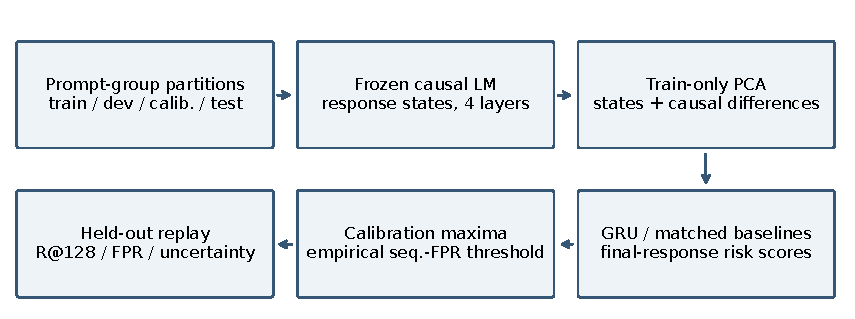
\includegraphics[width=.98\textwidth]{figures/architecture.pdf}}{\fbox{架构图等待报告生成。}}
\caption{实验数据流。检测器特征仅由训练记录拟合，测试标签不参与模型或阈值选择；测试文本只在已说明的语料构建重复审计中使用。示意图连接各实验阶段及其工件。}
\label{fig:architecture}
\end{figure*}

系统围绕三个连续环节展开。首先，分组数据准备与因果抽取确定每个检查点能够使用的信息；其次，降维投影与匹配检测器检验这些信息的表示和聚合方式；最后，序列级校准与缓冲释放将分数转化为运行决策。这条链路将预测问题、对照实验和在线接口连接起来。

\subsection{数据清洗与分组划分}
主数据来源为BeaverTails的30k训练分区。配置中的目标分配为8,000条训练回答、1,000条开发回答和1,000条校准回答，实际分配还受到样本合格条件与提示分组约束。官方测试分区中所有保留的合格回答构成主测试集。这些数字是研究设计配额；实际保留数量由处理后文件生成，见表~\ref{tab:dataset}。

规范化记录保存标识符、标准化提示分组、分区、来源、回答标签、可用类别、文本、token标识序列和回答长度。按标准化提示分组避免同一标准化问题的多个回答跨越分区。官方测试具有保留优先级，与其提示或回答模板匹配的记录从候选训练池移除。字符TF--IDF最近邻比较还在相似度0.92处移除接近测试提示的候选提示组；这一仅文本审计变换不被检测器复用，也不读取测试标签。训练、开发与校准之间进一步隔离精确相同的回答模板。保留样本标识符与来源版本，使这些决定可独立于训练检查。

配置限制提示长度不超过256个token、回答长度不超过512个token，均以固定分词器计数。超过长度限制的回答被排除，不采用静默截断后继续沿用完整回答标签的方式。这样保留了完整回答与原始标签的关系，但也使研究对象偏向较短回答。因此，性能结果必须同时报告长度排除和类别计数。空记录与非法记录被拒绝；某一类别缺失时，相应指标保持未定义，不生成虚构估计。

外部数据使用原始StreamGuardBench的\texttt{wildguard\_qwen3\_8b}测试分区，以不可变revision标识~\cite{streamguardbench2025data}。准备过程保留原始回答标签，预测输入采用提示和回答前缀。重复冲突优先保留留出测试记录，版本、排除项及保留标识均由审计保存。

\begin{table}[t]
\centering\footnotesize
\caption{长度筛选、分组和去重后实际保留的回答。}\label{tab:dataset}
\begin{tabular}{lrrr}\toprule
Split & $N$ & Unsafe & Groups \\
\midrule
calibration & 1001 & 563 & 275 \\
dev & 1003 & 551 & 282 \\
external & 591 & 54 & 591 \\
test & 3018 & 1732 & 2524 \\
train & 7997 & 4560 & 2211 \\
\bottomrule\end{tabular}
\end{table}

合格条件审计在1,725条外部回答中保留591条（34.3\%），其中原始284条不安全回答保留54条，保留样本的不安全比例为9.1\%。排除原因与类别保留比例由审计和图形源数据共同记录。

\resultfigure{data_class_balance}{保留回答的类别组成。计数单位为回答，提示组数量另见表~\ref{tab:dataset}。图中为描述性比例，不提供假定回答独立的置信区间。}{数据组成等待处理后记录。}
\resultfigure{external_retention}{外部测试来源经合格条件筛选后的按类别保留比例。标签显示保留数与原始数，差异性保留改变了评估总体。}{外部合格条件审计尚未完成。}

\subsection{冻结因果特征抽取}
特征骨干为Qwen2.5-0.5B-Instruct~\cite{qwen2024qwen25}，其权重保持冻结，FP16抽取降低激活存储开销。选取返回隐状态的第6、12、18和24个索引，最后一个索引包含骨干末端RMSNorm。各分区固定提示模板和分词器身份。抽取遵循因果注意力结构，使某一回答位置的表征仅依赖其提示与已可见回答上下文。

教师强制回放在因果注意力下计算记录回答的监测表征。外部Qwen3-8B回答由冻结的Qwen2.5监测模型编码，回答生成来源与表征提取模型分别记录，从而支持受控的检测器比较。

原始特征按照四个回答token的基础步长缓存，必要时追加最终token。主检测器步长为八，步长四和十六的变体复用同一缓存。该设计将代价较高的骨干抽取与相对便宜的检测器比较分离。缓存元数据记录层顺序、token位置与预处理身份，避免检测器静默读取与训练不一致的表征。

\subsection{增量PCA与时序特征工程}
设$h^{(\ell)}_{i,t}\in\mathbb R^d$为第$\ell$层的因果隐状态。增量主成分分析（PCA）只使用训练回答拟合64维投影。PCA通过正交的高方差方向概括协方差结构~\cite{jolliffe2016pca}，分批拟合适合检查点观测的内存受限处理；其作用是为后续监督分类构造紧凑的无监督表示。每条训练回答最多抽取八个检查点用于拟合，限制长回答的贡献。少于64行的末尾拟合批被省略并记录于元数据，但其中回答仍参与后续变换和检测器训练。每层分别处理：
\begin{equation*}
 z^{(\ell)}_{i,t}=\operatorname{diag}(\max(\lambda_\ell,\epsilon))^{-1/2}
 P_\ell(h^{(\ell)}_{i,t}-\mu_\ell).
\end{equation*}
其中$\lambda_\ell$为训练解释方差，通过除以其平方根对白化投影状态，并使用数值下限$\epsilon=10^{-8}$。拟合的均值、投影和方差保持不变，用于开发、校准及两个测试分区。本研究采用归纳设置；即使不读取标签，在合并数据集上拟合PCA也会引入传导式依赖。

\PCAVarianceZH{}

每个选定层拼接白化状态$z_t$、差分$z_t-z_{t^-}$、余弦变化$1-\cos(z_t,z_{t^-})$及范数变化$\|z_t\|_2-\|z_{t^-}\|_2$。四层输入共$4(64+64+1+1)=520$维，最后一层消融为130维。首次检查点的所有变化特征均为零。改变步长时，在实际选择的检查点之间重新计算差分，而不从另一步长的差分中直接子采样。特征缩放同样只在训练检查点拟合，并采用回答均衡样本权重。这样，每项依赖数据的变换都位于验证与阈值选择之前。

\subsection{检测器与匹配基线}
主要时序模型是隐藏维数为64的单层单向GRU，并接线性标量输出。对于特征向量$x_{i,t}$与循环状态$s_{i,t}$，
\begin{equation*}
 s_{i,t}=\operatorname{GRU}(x_{i,t},s_{i,t^-}),\quad
 \risk_{i,t}=\sigma(w^\top s_{i,t}+b),
\end{equation*}
其中$t^-$表示上一检查点。每条回答开始时重置循环状态；右侧padding不参与监督和评估，也不会影响单向网络已经产生的有效前缀输出。

四项基线分别检验不同解释。仅提示逻辑回归衡量在读取回答前能够预测的风险。前缀TF--IDF逻辑回归使用提示与当前可见回答文本，词和字符词表只由训练集拟合。当前状态逻辑回归检验当前降维表征是否足够，历史均值逻辑回归检验没有学习型循环记忆时的因果聚合。所有模型采用相同最终回答目标和评估规则。

文本表征拼接词1--2-gram与词内字符3--5-gram，每部分至多20,000维，采用次线性词频。线性模型使用$C=1$、按回答计数的类别平衡权重及liblinear求解器，迭代上限为500次。

消融分别移除变化特征、只保留最后一个选定层、以只观察当前检查点的多层感知机（MLP）替换GRU，或改变检查步长。动态GRU与仅状态GRU的差异对应新增特征的价值；动态GRU与动态MLP的差异对应循环聚合的价值。各变体在共同数据与校准规则下刻画特征构造和聚合选择。

\subsection{增量监测接口约定}
在线接口先消费token，再计算对应检查点状态。当前块保持缓冲，未告警时释放，告警时丢弃并停止生成；EOS前不足间隔的尾块同样检查，每条回答均重置检测器和特征构造器状态。

\section{训练、校准与不确定性}\label{sec:protocol}
\subsection{回答均衡的弱前缀监督}
每条训练回答最多选择八个等距检查点贡献监督损失，包含回答终点。若$\mathcal S_i$为选中的检查点集合，神经模型目标为
\begin{equation}
 \mathcal L=\frac{1}{N}\sum_{i=1}^N\frac{1}{|\mathcal S_i|}
 \sum_{t\in\mathcal S_i}\operatorname{BCE}_{w_+}(a_{i,t},Y_i),
 \label{eq:loss}
\end{equation}
其中$a$是sigmoid之前的logit，$w_+=N_0/N_1$为正类回答权重。内部平均避免长回答仅因检查点更多而获得更大损失权重。线性模型也采用检查点数倒数样本权重，并按回答计数设置类别权重。

式~\ref{eq:loss}实现面向最终结局的回答均衡弱前缀监督。各检查点预测同一目标，结合仅提示控制与回答特征消融，刻画不同可见信息的贡献。

神经模型使用AdamW，配置学习率为$10^{-3}$、权重衰减为$10^{-4}$，批大小32，梯度裁剪上限1.0，训练最多20轮。以开发集回答最大分数的ROC AUC选择检查点，早停耐心值为三。随机种子13、42和2026在实验前固定。开发集用于选择模型状态，独立校准集用于确定操作阈值；测试测量不参与这两项选择。

\subsection{经验序列级校准}
对每条安全校准回答定义$M_i=\max_t\risk_{i,t}$，将其$n_0$个值排序为$M_{(1)}\leq\cdots\leq M_{(n_0)}$。给定目标$\alpha=0.05$以及$k=\lfloor\alpha n_0\rfloor$，实现中的阈值为
\begin{equation*}
 \tau=M_{(n_0-k)}.
\end{equation*}
在严格大于的告警规则下，至多$k$条安全校准回答超过阈值；并列值可使经验误报率更低。测试阶段同时报告相应召回率和实际序列误报率。

每种方法、每个种子使用相同校准过程和目标获得各自阈值，以适应评分尺度差异；外部评价沿用已拟合检测器及其域内阈值。

\subsection{分组配对估计}
点估计采用固定种子间的均值与样本标准差汇总。重采样以提示分组为单位，保留同题回答之间的内容和难度关联。

配对bootstrap有放回抽取提示组1,000次，保留所选组内全部回答，并对比较双方及其共同种子使用相同抽样。分数和阈值固定，差值为待比较方法减去参考方法，95\%百分位区间采用2.5\%和97.5\%分位数。

Recall@128定义主对照；次要指标、消融与探索性敏感性分析在表格中分别标识，并与完整逐种子测量一同归档。

\section{实验结果}\label{sec:results}
结果依次回答三个研究问题，再报告系统测量和探索性表征分析。各方法采用共同的5\%校准目标，并结合实际测试误报率解释召回表现。
\subsection{RQ1：表征与检测器选择}
\paragraph{完整流程比较。}\AchievementDetectionZH{} 提示分组配对不确定性见表~\ref{tab:uncertainty}。

\begin{table}[t]
\centering\footnotesize
\caption{域内检测结果（百分比）。报告可用种子的均值与样本标准差；单种子不显示标准差。阈值仅依据域内校准集确定。}\label{tab:main}
\begin{tabular}{lrrrr}\toprule
Method & R@128 & FPR & AUROC & AP \\
\midrule
Prompt LR & 22.9 $\pm$ 0.0 & 3.3 $\pm$ 0.0 & 74.4 $\pm$ 0.0 & 80.1 $\pm$ 0.0 \\
Prefix TF--IDF LR & 28.2 $\pm$ 0.0 & 1.6 $\pm$ 0.0 & 81.1 $\pm$ 0.0 & 86.3 $\pm$ 0.0 \\
Current-state LR & 43.7 $\pm$ 0.0 & 5.6 $\pm$ 0.0 & 83.1 $\pm$ 0.0 & 86.5 $\pm$ 0.0 \\
Running-mean LR & 46.1 $\pm$ 0.0 & 6.2 $\pm$ 0.0 & 83.5 $\pm$ 0.0 & 86.5 $\pm$ 0.0 \\
Dynamic GRU & 38.1 $\pm$ 6.3 & 3.3 $\pm$ 1.0 & 83.6 $\pm$ 0.9 & 87.6 $\pm$ 0.8 \\
\bottomrule\end{tabular}
\end{table}


\paragraph{检测器权衡。}表~\ref{tab:main}完整呈现基线比较。静态探针、MLP和循环头在共同校准目标下形成互补的召回率—误报率运行特征，为应用选择检测器提供依据。

\begin{table}[t]
\centering\footnotesize
\caption{域内告警位置；位置统计以正确检出为条件，召回率分母保留所有不安全回答。}\label{tab:alert_positions}
\begin{tabular}{lrrrr}\toprule
Method & Recall & Mean $\tau$ & Med. $\tau$ & $\tau/T$ (\%) \\
\midrule
Prompt LR & 22.9 $\pm$ 0.0 & 8.0 $\pm$ 0.0 & 8.0 $\pm$ 0.0 & 14.8 $\pm$ 0.0 \\
Prefix TF--IDF LR & 28.3 $\pm$ 0.0 & 20.7 $\pm$ 0.0 & 8.0 $\pm$ 0.0 & 26.2 $\pm$ 0.0 \\
Current-state LR & 43.9 $\pm$ 0.0 & 27.5 $\pm$ 0.0 & 16.0 $\pm$ 0.0 & 34.6 $\pm$ 0.0 \\
Running-mean LR & 46.3 $\pm$ 0.0 & 15.1 $\pm$ 0.0 & 8.0 $\pm$ 0.0 & 23.5 $\pm$ 0.0 \\
Dynamic GRU & 38.4 $\pm$ 6.1 & 47.9 $\pm$ 15.1 & 41.8 $\pm$ 18.3 & 54.0 $\pm$ 11.5 \\
\bottomrule\end{tabular}
\end{table}


\begin{table}[t]
\centering\footnotesize
\caption{提示分组配对自助法：Recall@128差值及95\%区间（百分点）。}\label{tab:uncertainty}
\begin{tabular}{lp{.34\columnwidth}rr}\toprule
Split & Contrast & $\Delta$ & 95\% CI \\
\midrule
test & Dynamic GRU vs. Prompt LR & +15.2 & [+12.7, +17.8] \\
test & Dynamic GRU vs. Current-state LR & -5.6 & [-7.1, -3.9] \\
test & Dynamic GRU vs. Prefix TF--IDF LR & +9.9 & [+7.6, +12.2] \\
external & Dynamic GRU vs. Prompt LR & +12.3 & [+6.7, +18.8] \\
external & Dynamic GRU vs. Current-state LR & -11.7 & [-20.6, -3.6] \\
external & Dynamic GRU vs. Prefix TF--IDF LR & +12.3 & [+6.7, +18.8] \\
\bottomrule\end{tabular}
\end{table}


\paragraph{同题不同结局。}测试集中同一问题同时存在两种最终标签的子集包含97组、207条回答。冻结阈值下，动态GRU与当前状态逻辑回归的Recall@128分别为20.1\%和22.3\%，误报率分别为6.1\%和6.7\%。这一同题子集刻画了两种检测器在共享问题、不同回答结局下的表现。

\paragraph{历史聚合对照。}历史均值逻辑回归的Recall@128为46.1\%，动态GRU相对差值为-8.1个百分点。该对照量化因果历史积累的作用，补充当前状态与学习式循环模型的比较。

\paragraph{不确定性。}表~\ref{tab:uncertainty}保留提示分组配对自助法区间。每次配对抽样在检测器之间保留一致的提示分组和已拟合种子。

\paragraph{预设对照。}动态GRU减去静态探针的Recall@128差值为-5.64个百分点，提示分组95\%区间为[-7.10, -3.93]。静态探针侧重召回覆盖，GRU则具有较低实测误报率，两类运行特征对应不同监测需求。

\paragraph{补充排序与校准。}

\ReviewRankingZH{} AUROC@128采用预算内检查点的最大分数，区间通过1,000次提示分组配对bootstrap计算。该线性分类器家族内的比较，为不同特征构造提供了补充排序证据。

GRU与静态探针具有接近的预算内排序表现，AUROC@128差值为0.0050，95\%区间为[-0.0019, 0.0123]。

表~\ref{tab:review_sensitivity}比较1\%、5\%和10\%校准目标下的运行特征；已拟合模型固定，原5\%目标保留为主设定。\begin{table}[t]
\centering\footnotesize
\caption{事后探索性校准目标分析；数值为三个固定种子均值（百分比）。阈值由校准集确定，5\%为主设定；比较区间未作多重校正。}\label{tab:review_sensitivity}
\begin{tabular}{lrrr}\toprule
Method & $\alpha$ & R@128 & Test FPR \\
\midrule
Prefix TF--IDF LR & 1 & 12.9 & 0.3 \\
Current-state LR & 1 & 18.0 & 1.2 \\
Dynamic GRU & 1 & 18.5 & 1.0 \\
Prefix TF--IDF LR & 5 & 28.2 & 1.6 \\
Current-state LR & 5 & 43.7 & 5.6 \\
Dynamic GRU & 5 & 38.1 & 3.3 \\
Prefix TF--IDF LR & 10 & 43.7 & 5.5 \\
Current-state LR & 10 & 61.7 & 13.5 \\
Dynamic GRU & 10 & 56.2 & 9.0 \\
\bottomrule\end{tabular}
\end{table}


严格完成前检出要求告警检查点早于回答终点，且处于128-token预算内。以全部不安全回答为分母时，主测试静态探针和GRU的召回分别为42.8\%与35.1\%。这一时机视角补充了预算内召回曲线。


\resultfigure{recall_budget_test}{域内测试集在不同可见token预算下的不安全回答召回率。点和误差条分别表示已完成种子的均值与一个样本标准差，单种子不显示标准差，各方法保持阈值冻结。}{尚无完成的召回率曲线。}

\subsection{RQ2：检查频率与特征消融}
消融表与配图比较特征、聚合方式和检查步长。仅状态GRU保留循环结构并移除变化特征，动态MLP保留输入特征并替换记忆结构。步长比较同时改变下一个允许告警的时刻和评分次数，并按实际步长重新计算动态特征。这些对照在共同抽取与校准流程中，为系统配置提供选择依据。
\begin{table}[t]
\centering\footnotesize
\caption{Ablation and checkpoint-stride sensitivity (\%).}\label{tab:ablation}
\begin{tabular}{lrr}\toprule
Setting & R@128 & Seq. FPR \\
\midrule
Dynamic GRU & 38.1 $\pm$ 6.3 & 3.3 $\pm$ 1.0 \\
GRU, states only & 41.2 $\pm$ 3.2 & 3.3 $\pm$ 0.8 \\
GRU, last layer & 33.3 $\pm$ 0.9 & 2.7 $\pm$ 0.2 \\
Dynamic MLP & 47.7 $\pm$ 4.1 & 5.1 $\pm$ 1.2 \\
GRU, stride 4 & 40.5 $\pm$ 4.2 & 3.0 $\pm$ 0.9 \\
GRU, stride 16 & 37.0 $\pm$ 2.2 & 3.5 $\pm$ 0.2 \\
\bottomrule\end{tabular}
\end{table}

\resultfigure{ablations}{时序结构、特征和检查步长比较的实测Recall@128。条形和误差分别为已完成种子的均值与一个样本标准差，没有测量的设置不绘制。}{消融测量尚未完成。}

\subsection{RQ3：骨干规模与回答来源迁移}
规模实验固定回答划分并改变监测骨干，外部实验改变回答来源并沿用已经拟合的检测器和阈值。两者分别检验表征规模扩展与完整判决规则的迁移表现。
\AchievementScaleZH{}
\paragraph{骨干规模。}表~\ref{tab:scale}在相同回答划分上比较冻结的0.5B与1.5B表示。1.5B采用返回隐状态的第7、14、21和28个索引，每层降维维数与训练协议保持一致。两种配置编码相同的回答划分。\begin{table}[t]
\centering\footnotesize
\caption{相同样本下的骨干规模验证（百分比）；各规模使用独立训练与校准工件。}\label{tab:scale}
\begin{tabular}{llrrr}\toprule
Size & Method & R@128 & FPR & Ext. R@128 \\
\midrule
0.5B & Current-state LR & 43.7 $\pm$ 0.0 & 5.6 $\pm$ 0.0 & 24.1 $\pm$ 0.0 \\
0.5B & Dynamic GRU & 38.1 $\pm$ 6.3 & 3.3 $\pm$ 1.0 & 12.3 $\pm$ 13.4 \\
1.5B & Current-state LR & 54.0 $\pm$ 0.0 & 5.8 $\pm$ 0.0 & 25.9 $\pm$ 0.0 \\
1.5B & Dynamic GRU & 49.6 $\pm$ 4.6 & 4.9 $\pm$ 1.7 & 17.3 $\pm$ 2.8 \\
\bottomrule\end{tabular}
\end{table}


\begin{table}[t]
\centering\footnotesize
\caption{外部检测结果（百分比）。报告可用种子的均值与样本标准差；单种子不显示标准差。阈值仅依据域内校准集确定。}\label{tab:external}
\begin{tabular}{lrrrr}\toprule
Method & R@128 & FPR & AUROC & AP \\
\midrule
Prompt LR & 0.0 $\pm$ 0.0 & 4.7 $\pm$ 0.0 & 48.2 $\pm$ 0.0 & 8.2 $\pm$ 0.0 \\
Prefix TF--IDF LR & 0.0 $\pm$ 0.0 & 1.3 $\pm$ 0.0 & 62.0 $\pm$ 0.0 & 12.8 $\pm$ 0.0 \\
Current-state LR & 24.1 $\pm$ 0.0 & 8.6 $\pm$ 0.0 & 80.0 $\pm$ 0.0 & 31.0 $\pm$ 0.0 \\
Running-mean LR & 11.1 $\pm$ 0.0 & 2.6 $\pm$ 0.0 & 80.8 $\pm$ 0.0 & 27.8 $\pm$ 0.0 \\
Dynamic GRU & 12.3 $\pm$ 13.4 & 5.0 $\pm$ 1.1 & 81.0 $\pm$ 1.9 & 33.1 $\pm$ 4.4 \\
\bottomrule\end{tabular}
\end{table}


\paragraph{迁移边界。}外部评估使用冻结的域内阈值，考察完整评分与阈值规则能否迁移。来源模型、标注规则和回答长度的差异都可能造成迁移性能变化。
外部集上，种子13、42和2026的GRU在128-token预算内分别检出2, 15, 3条不安全回答，分母均为54。种子42为15/54，描述性Wilson 95\%区间为[17.6, 40.9]\%。归档同时提供逐种子召回和误报的计数与区间。

\resultfigure{recall_budget_external}{保持域内阈值不变时的外部早期召回率。误差条与域内图一致，表示一个种子标准差。此处评估回答来源变化下的回放迁移。}{外部测量尚未完成。}

\subsection{系统可行性与增量运行}
系统测量将检测研究连接到本机实践：共享缓存摊薄骨干抽取成本，检查点计时量化附加监测工作，增量回放核对离线与KV运行的评分一致性。
\begin{table}[t]
\centering\footnotesize
\caption{实测训练与检测头耗时；种子间取均值。头部延迟不含骨干、分词、PCA及动态特征构造。}\label{tab:timing}
\begin{tabular}{lrrr}\toprule
Method & Fit (s) & p50 (ms) & p95 (ms) \\
\midrule
Prompt LR & 5.44 & -- & -- \\
Prefix TF--IDF LR & 29.34 & -- & -- \\
Current-state LR & 5.67 & -- & -- \\
Running-mean LR & 5.37 & -- & -- \\
Dynamic GRU & 36.20 & 0.21 & 0.26 \\
GRU, states only & 34.16 & 0.21 & 0.26 \\
GRU, last layer & 42.33 & 0.20 & 0.28 \\
Dynamic MLP & 31.21 & 0.14 & 0.16 \\
GRU, stride 4 & 47.50 & 0.21 & 0.27 \\
GRU, stride 16 & 24.60 & 0.21 & 0.30 \\
\bottomrule\end{tabular}
\end{table}

\paragraph{等长生成开销。}对固定良性演示提示完成3组预热后的配对测量，无监测与仅监测生成的中位耗时分别为2.267和2.250秒，配对开销中位数为-0.1\%。每组贪心生成的token序列散列完全一致，耗时不包含模型加载。这一配对设计在相同生成工作负载中测量检查点监测开销。

配对比例的实测范围为-5.4\%至+6.2\%。配对测量显示，本机监测生成的耗时与无监测基线接近。

跨试验的检查点监测p50与p95时延中位数分别为0.82和0.89毫秒，仅监测生成的吞吐中位数为28.4 token/秒，PyTorch分配显存峰值为0.95 GiB。检查点计时包含特征构造和检测器推理，区别于仅检测头表格。

\paragraph{在线集成。}独立受控生成演示生成128个token，经检查点判决后释放128个，停止状态为false。该功能运行还结合确定性样例检验缓冲丢弃和EOS尾块处理。

受控生成耗时4.936秒，吞吐为25.9 token/秒。该运行完成了配置的生成预算。

\paragraph{冻结抽取成本。}主抽取记录在723.1秒内处理1,548,168个提示与回答token，吞吐为2141.0 token/秒，PyTorch分配显存峰值为0.99 GiB。显存采用PyTorch分配量口径，吞吐对应本机测量。

主实验原始隐状态与投影缓存分别占用1837.5和132.9 MiB，包含各自清单；冻结骨干权重不计入此缓存体积。
真实KV回放在6条留出回答的53个检查点上与离线分数对照，最大差值为0.00110，阈值判决不一致数为0。诊断采用每种标签按ID排序的前三条长度16--128回答和种子42的GRU。

\resultfigure{risk_trajectories}{从保存预测中确定性选择的去标识示例轨迹。颜色标识最终回答标签，曲线沿已观察检查点展开。}{预测轨迹尚不可用。}

\subsection{PCA可视化与K均值聚类分析}
探索性分析通过无监督模式发现补充监督预测。第二次PCA用于展示训练终点的二维分布，K均值则依据簇内平方距离在完整降维表征中形成分组~\cite{lloyd1982quantization}；比较各簇的最终标签构成，可以描述回答风险在不同表征群体中的分布。
展示用PCA仅在7,997个保留训练终点上拟合，二维保留其28.9\%方差。K均值在完整256维降维终点空间中无标签拟合八类；外部终点可用时，通过冻结中心分配类别。无监督拟合完成后，再利用标签描述各簇的风险构成。终点分析展示整体表征结构，与前缀分类实验形成互补。\begin{table}[t]
\centering\footnotesize
\caption{事后训练集拟合的终点聚类。风险比例为描述性百分比，聚类编号没有顺序含义。}\label{tab:clusters}
\begin{tabular}{rrrrr}\toprule
Cluster & Train $N$ & Unsafe & Ext. $N$ & Unsafe \\
\midrule
0 & 703 & 58.7 & 269 & 10.8 \\
1 & 1496 & 44.1 & 70 & 20.0 \\
2 & 1522 & 53.0 & 125 & 5.6 \\
3 & 1107 & 60.9 & 1 & 0.0 \\
4 & 316 & 77.8 & 15 & 0.0 \\
5 & 1711 & 78.8 & 2 & 0.0 \\
6 & 769 & 21.5 & 5 & 20.0 \\
7 & 373 & 66.5 & 104 & 2.9 \\
\bottomrule\end{tabular}
\end{table}


\resultfigure{pca_endpoints}{所有保留训练终点的训练集限定PCA展示。投影使用全部保留训练终点拟合，颜色标识最终回答标签，点顺序采用固定随机置换。}{探索性PCA等待完整训练特征缓存。}
\resultfigure{cluster_composition}{八个训练集拟合终点聚类内不安全回答的描述性比例。K均值使用全部降维状态维度，外部样本沿用相同中心；源数据同时提供样本和提示组计数。}{聚类探索等待降维终点特征。}

\section{讨论与研究展望}
\subsection{表征挖掘与检测器选择}
实验将紧凑隐状态表征与实际检测器选择联系起来。在共同校准规则下，静态探针侧重回答覆盖，GRU则处于较低实测误报率的运行点；MLP与仅状态对照进一步区分了特征构造和序列聚合的作用。这些运行特征为应用按召回、误报和资源要求选择检测器提供了依据。

后续可引入容量匹配的仅提示神经网络，并采用相同优化预算开展因子化比较。当前prompt到GRU的对照同时改变了表征与分类结构，此类实验将更精细地区分两者贡献。结合表征干预与来源均衡的研究，还可进一步分析拒绝风格、回答长度及语义风险相关线索。

\subsection{风险类别覆盖与数据拓展}
\paragraph{描述性误差分层。}在不安全测试回答至少30条的类别中，全流平均召回率最低的三个类别为：controversial topics, politics: 6.0\% ($N=95$); sexually explicit, adult content: 22.0\% ($N=103$); discrimination, stereotype, injustice: 24.4\% ($N=297$)。这些多标签描述统计为分类别数据收集与后续分析提供方向。

\paragraph{可追溯案例。}误差归档保留案例beavertails-91be36a1f68f4cf9da034fa4, beavertails-b28c850e93be35ebdd9c1358：在两类错误均存在时，分别对应种子42中最高分误报与最低分漏报。这些确定性选择的诊断案例可以通过来源标识进一步核查。

这些类别差异为低召回风险领域的定向收集与标注提供了方向。当前英文样本采用256个prompt token和512个response token的长度限制，外部测试保留54条不安全回答。面向更长回答、更多生成来源和多语言内容扩展数据，将支持更细致的迁移估计和类别分析；结合长度分层采样与一致标注规则，有助于区分来源变化和回答构成的影响。

\subsection{从回答风险预测到原生生成干预}
当前监督描述完整回答的最终安全性，监测状态通过因果回放提取。\TimingProfileZH{} 后续可结合人工前缀标注与独立标注的原生生成回答，将回答级预测、危害起点定位和面向用户的释放决策纳入统一评价设计。

缓冲接口与KV数值诊断为这一方向提供了工程基础。通过随机化停止／继续生成对照、扩大回答长度覆盖和重复端到端计时，可以进一步刻画安全性—可用性权衡及部署尾时延。现有良性生成示例和六回答数值诊断提供了实现层面的功能证据，下一阶段将进一步测量干预结果。

\subsection{校准与可复现泛化}
经验校准目标用于设定运行规则，实际测试误报率用于描述该规则在留出回答上的表现；分组bootstrap区间刻画已拟合系统的评估样本波动。进一步重复训练和校准重采样、扩大外部样本，以及引入风险控制校准，可将不确定性分析拓展至新的研究总体。基础模型数据污染审计还将补充分组隔离之外的来源追溯。

项目归档了配置、预处理器、模型状态、阈值和逐回答轨迹，两份文稿共享数值来源。这套工件结构支持持续比较，使新数据、检测头与校准策略能够接入同一因果特征和报告约定。

\section{结论}
流式回答风险预测需要有效的前缀特征、面向整段回答的判决规则，以及可负担的重复推理成本。本文通过数据清洗、仅训练集增量PCA、时序特征工程、轻量序列分类和连接缓冲生成的序列级校准，形成对应的解决方案；K均值与二维PCA进一步概括回答表征的群体结构。\ReviewRankingZH{} 检测器比较给出明确的实践选择：静态探针侧重召回覆盖，GRU则运行于较低的实测误报率。检查步长消融量化监测频率对覆盖的影响，规模实验进一步展示扩大冻结骨干对静态探针的作用。\AchievementScaleZH{} 共享缓存与增量运行实测使该流程能够在本机资源条件下实施。后续将沿用同一可复现框架，拓展前缀标注、来源覆盖与原生生成评价。

\appendices
\section{复现与工件约定}
复现采用分阶段命令入口和冻结配置签名；不兼容的缓存、预处理器、权重或阈值均被拒绝。预测行保留回答ID、提示分组、标签、检查点位置与分数，配对估计先核对记录对齐再重采样。两稿共享数值工件、矢量图、源数据和参考文献，并通过SHA-256清单连接至归档测量。接口约定、统计边界情况和执行步骤由代码、单元测试及复现指南覆盖。

\bibliographystyle{IEEEtran}
\bibliography{refs}
\end{document}
